\chapter{Geheugenarchitectuur}
\label{architecture}
De afzonderlijke geheugencellen zullen uiteindelijk samengebracht moeten worden in een geheel.
In dit hoofdstuk zal de algemene structuur besproken worden alsook de vrijheidsgraden die in hoofdstuk \ref{timing-optimization} onderzocht worden voor een optimaal werkend systeem. Ten slotte zullen ook nog de bouwblokken aangekaard worden die meer uitvoerig besproken worden in de volgende hoofdstukken. 

\section{Van transistorniveau tot systeemniveau}
Hoewel het hele systeem op de chip in weze bestaat uit transistoren en passieve componenten, zal dit nog onmogelijk te begrijpen vallen op zulke grote schaal.
Het is daarom aangewezen om meer abstractie te maken en de componenten vanop een hoger niveau te bekijken.

\subsection{Cel}
Zoals besproken in hoofdstuk \ref{cell} zal dit het bouwblok zijn dat het vaakst terug zal te vinden zijn op het geheugensysteem.
De cel bestaat uit een memristor en een transistor. De geheugencel heeft drie terminals: de gate van de transistor, die zal verbonden worden met een wordline, de source van de transistor, die zal verbonden worden met een sourceline en tenslotte de terminal van de memristor, die zal verbonden worden met een bitline.
Een cel wiens memristor zich in een willekeurige resistieve staat bevindt is een datacel, terwijl de memristor van referentiecellen in een voorgeprogrammeerde en dus gekende resistieve staat verkeert.

\subsection{Branch}
In een branch worden er een bepaald aantal datacellen verbonden aan één BL en één SL. Dit aantal wordt \emph{Number of Word Lines per Branch} (NoWLpB) genoemd en is een van de vrijheidsgraden van de geheugenarchitectuur. Naast alle datacellen is er ook nog één referentiecel verbonden aan de BL en SL van de branch.
Elke BL wordt via een pMOS-transistor verbonden met de voedingspanning Vdd en via een nMOS-transistor aan de grondspanning Vss. In dit werk is er enkel een nMOS-transistor die de SL verbindt met Vss.\footnote{In een volledig geheugensysteem zou de SL via een pMOS ook nog verbonden zijn met een niet onderzochte spanningsknoop Vdd\_write. De pMOS zou dan worden aangezet voor schrijfwerking.} De nMOS-transistoren aan BL en SL fungeren als schakelaars, de pMOS-transistor wordt gebruikt als impedantie voor een resistieve spanningsdeling (zie hoofdstuk \ref{loadanalysis}).
Ter illustratie wordt de samenhang tussen cel en branch getoond in figuur \ref{fig:cellbranch}.

\begin{figure}
  \centering
  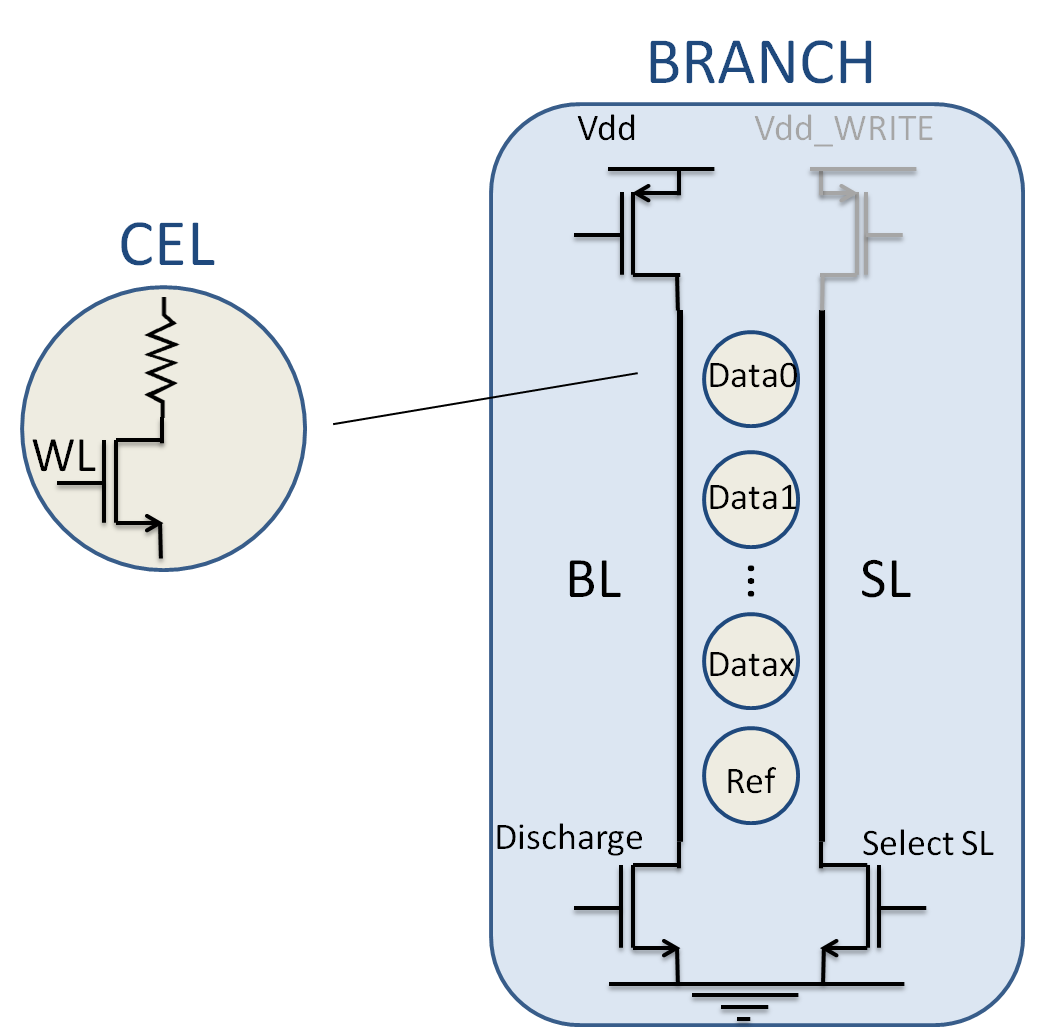
\includegraphics[scale=0.3]{../fig/hfdstk-architecture-cell-branch.png}
  \caption{Een geheugencel en een branch}
  \label{fig:cellbranch}
\end{figure}

\subsection{Local Block}
Verschillende BLs en SLs worden samengebracht in een Local Block, waarvan de vrijheidsgraad \emph{Number of Bit Lines per Local Block} (NoBLpLB) heet. In een LB bevinden er zich dus NoBLpLB x NoWLpB datacellen en NoBLpLB referentiecellen. Ook zitten er in een Local Block zowel BL- als WL-decoders.
De structuur van een Local Block is geïllustreerd op figuur \ref{fig:LB}.
De uitgangen van de WL-decoder zullen (mits wat buffering tussenin) worden aangesloten aan de data-WLs zelf, die van de BL-decoder zullen een spanningsdeling teweeg brengen op de BLs. De referentie-WL zal via een extern signaal verbonden worden.
Aangezien een LB zowel data- als referentiecellen bevat, gaat een LB twee werkingsmodes hebben: een mode waarbij er één datacel wordt aangesproken en een mode waarbij er een bepaald aantal referentiecellen in parallel wordt aangesproken.

\begin{figure}
  \centering
  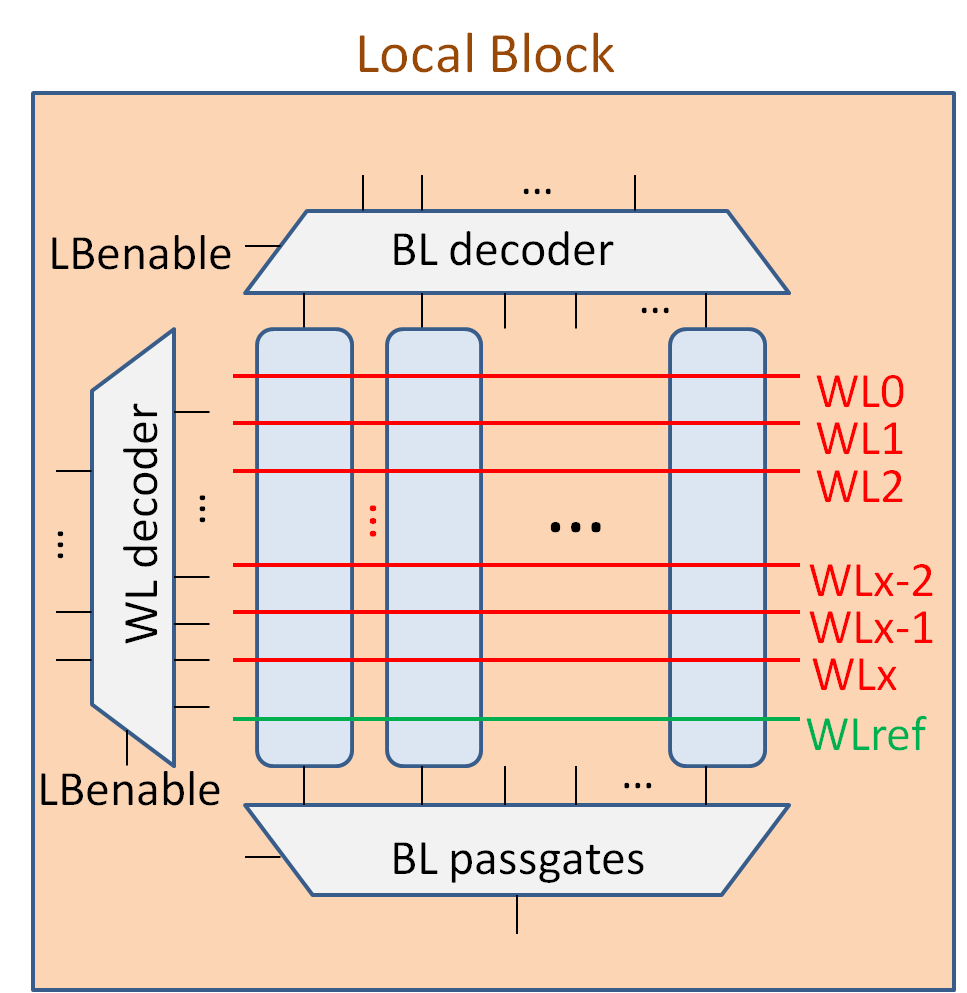
\includegraphics[scale=0.3]{../fig/hfdstk-architecture-localblock.png}
  \caption{Een Local Block}
  \label{fig:LB}
\end{figure}

\subsection{Global Block}
Een Global Block bestaat uit twee LBs en een sense amplifier (SA). In het ene LB gaat er een datasignaal geproduceerd worden, in het andere een referentiesignaal (zie figuur \ref{fig:GB}. Vervolgens gaat de SA dit kleine signaalverschil versterken tot een zuivere rail-to-rail output.
Aan de uitgang van het GB verschijnen dan ook de opgevraagde bits.
De laatste architectuurvrijheidsgraad is de \emph{Number of Global Blocks} (NoGB), het totale geheugen bevat dus NoGB x 2 x NoBLpLB x NoWLpB geheugencellen.

\begin{figure}
  \centering
  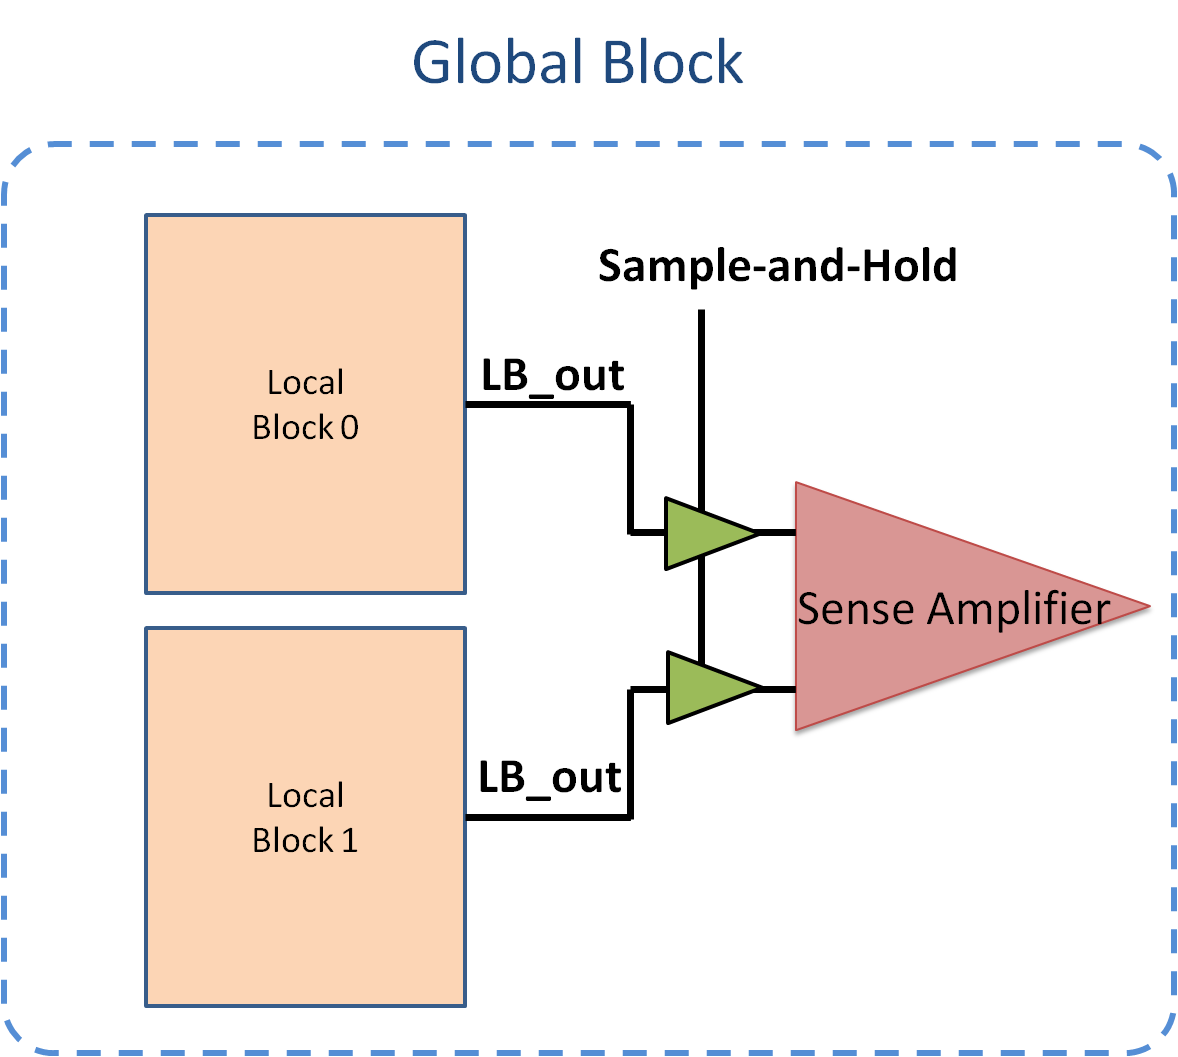
\includegraphics[scale=0.3]{../fig/hfdstk-architecture-globalblock.png}
  \caption{Een Global Block}
  \label{fig:GB}
\end{figure}

\section{Besluit}


